%%%%%%%%%%%%%%%%%%%%%%%%%%%%%%%%%%%%%%%%%
% Journal Article
% LaTeX Template
% Version 1.4 (15/5/16)
%
% This template has been downloaded from:
% http://www.LaTeXTemplates.com
%
% Original author:
% Frits Wenneker (http://www.howtotex.com) with extensive modifications by
% Vel (vel@LaTeXTemplates.com)
%
% License:
% CC BY-NC-SA 3.0 (http://creativecommons.org/licenses/by-nc-sa/3.0/)
%
%%%%%%%%%%%%%%%%%%%%%%%%%%%%%%%%%%%%%%%%%

%----------------------------------------------------------------------------------------
%	PACKAGES AND OTHER DOCUMENT CONFIGURATIONS
%----------------------------------------------------------------------------------------

\documentclass[twoside,twocolumn]{article}

\usepackage{blindtext} % Package to generate dummy text throughout this template 

\usepackage[sc]{mathpazo} % Use the Palatino font
\usepackage[T1]{fontenc} % Use 8-bit encoding that has 256 glyphs
\linespread{1.05} % Line spacing - Palatino needs more space between lines
\usepackage{microtype} % Slightly tweak font spacing for aesthetics

\usepackage[english]{babel} % Language hyphenation and typographical rules

\usepackage[hmarginratio=1:1,top=32mm,columnsep=20pt]{geometry} % Document margins
\usepackage[hang, small,labelfont=bf,up,textfont=it,up]{caption} % Custom captions under/above floats in tables or figures
\usepackage{booktabs} % Horizontal rules in tables

\usepackage{lettrine} % The lettrine is the first enlarged letter at the beginning of the text

\usepackage{enumitem} % Customized lists
\setlist[itemize]{noitemsep} % Make itemize lists more compact

\usepackage{abstract} % Allows abstract customization
\renewcommand{\abstractnamefont}{\normalfont\bfseries} % Set the "Abstract" text to bold
\renewcommand{\abstracttextfont}{\normalfont\small\itshape} % Set the abstract itself to small italic text

\usepackage{titlesec} % Allows customization of titles
\renewcommand\thesection{\Roman{section}} % Roman numerals for the sections
\renewcommand\thesubsection{\roman{subsection}} % roman numerals for subsections
\titleformat{\section}[block]{\large\scshape\centering}{\thesection.}{1em}{} % Change the look of the section titles
\titleformat{\subsection}[block]{\large}{\thesubsection.}{1em}{} % Change the look of the section titles

\usepackage{fancyhdr} % Headers and footers
\pagestyle{fancy} % All pages have headers and footers
\fancyhead{} % Blank out the default header
\fancyfoot{} % Blank out the default footer
\fancyhead[C]{Seminar Data Science \& Artificial Intelligence $\bullet$ SS25 proceedings} % Custom header text
\fancyfoot[RO,LE]{\thepage} % Custom footer text

\usepackage{titling} % Customizing the title section

\usepackage{hyperref} % For hyperlinks in the PDF

\usepackage{listings}
\usepackage{xcolor} % Für Farben (optional)
\lstdefinelanguage{pseudocode}{
    keywords={for, to, from, set, with, one, and, collect, update, using, end},
    keywordstyle=\color{blue}\bfseries,
    comment=[l]{//},
    morecomment=[s]{/*}{*/},
    morestring=[b]",
    sensitive=false
}

\lstset{
    language=pseudocode,
    basicstyle=\scriptsize\ttfamily,  % kleiner Code
    keywordstyle=\color{blue},
    commentstyle=\color{gray},
    mathescape=true,
    frame=single,
    backgroundcolor=\color{gray!5},
}

%----------------------------------------------------------------------------------------
%	TITLE SECTION
%----------------------------------------------------------------------------------------

\setlength{\droptitle}{-4\baselineskip} % Move the title up

\pretitle{\begin{center}\Huge\bfseries} % Article title formatting
\posttitle{\end{center}} % Article title closing formatting
\title{Sim-to-Real in Reinforcement Learning Across Multiple Domains} % Article title
\author{%
\textsc{Tim Knudsen} \\[1ex] % Your name
\normalsize FH Wedel University of Applied Sciences\\ % Your institution
\normalsize \href{tim04knudsen@gmail.com}{tim04knudsen@gmail.com} % Your email address
}
\date{\today} % Leave empty to omit a date
\renewcommand{\maketitlehookd}{%
\begin{abstract}
\noindent Reinforcement Learning is a modern and powerful approach to machine learning. It has achived remarkable success in simulated environments. But no matter how powerful your algorithm is, it is only as good as the deployment in the real world. Due to the complexity of the real world, the Sim-2-Real transfer is a major challenge in the field of Reinforcement Learning. In this paper, we will discuss the challenges of the Sim-2-Real transfer and how to overcome them. We will discuss different approaches to the Sim-2-Real transfer and how they can be used to improve the performance of Reinforcement Learning.
\end{abstract}
}

%----------------------------------------------------------------------------------------

\begin{document}

% Print the title
\maketitle
%----------------------------------------------------------------------------------------
\section{Introduction}
Reinforcement Learning (RL) has achieved remarkable results in simulated environments (e.g.\ video games, simulated robotics) but often fails to generalize to real-world systems due to the \emph{\simtoreal gap}. Simulation can provide abundant and safe data, yet differences in visual perception, physical dynamics, and task specifics cause learned policies to degrade in reality {\cite{Tobin2017,Sadeghi2017}}. For instance, a policy that navigates hallways with randomized CAD renderings can transfer to a real drone (CAD2RL {\cite{Sadeghi2017}}), and a humanoid robot hand can solve a Rubik’s cube in reality after training with Automatic Domain Randomization (ADR) in simulation {\cite{Akkaya2019}}. Nevertheless, open challenges remain: how to systematically reconcile each aspect of the Markov Decision Process (observations, actions, transitions, rewards) between sim and real. 

This paper revises and streamlines the literature through the Observation–Action–Transition–Reward (OATR) lens. We define each MDP component and describe how discrepancies in that component contribute to the transfer challenge. We then review \simtoreal methods aligned to each OATR category, emphasizing practical examples and empirical findings (e.g.\ Fig.~\ref{fig:adr_pipeline}, Fig.~\ref{fig:adapt_sim}). In each section, we critically evaluate techniques (such as domain randomization versus system identification for dynamics) and highlight gaps. Our goal is to provide a clear, concise master’s-level overview: by focusing on OATR, readers can identify which aspects of sim or real must be bridged and which methods apply. The remainder is organized into Observation-, Action-, Transition-, and Reward-focused transfer.

\section{Background}
\subsection{Definition}
An RL task is an MDP characterized by observation (state) $s$, action $a$, transition $T(s,a\to s')$, and reward $r$. In simulation, these are often idealized: perfect sensors, discretized actions, deterministic physics, and easily computable rewards. In reality, by contrast, sensors produce noisy observations, actuators have latency and limits, dynamics are stochastic and hard to model, and rewards may be sparse or indirect. Table~\ref{tab:elements} summarizes typical sim-versus-real discrepancies. Any of these mismatches can cause failure: for example, a vision policy may overfit simulated textures and fail on real images, or an action sequence learned without actuator latency may be unsafe on hardware.

\begin{table}[htbp]
    \centering
    \caption{Simulated vs real MDP components: sources of discrepancy (simulated vs real).}
    \begin{tabular}{|p{0.3\linewidth}|p{0.6\linewidth}|}
        \hline
        \textbf{Observation:} & Idealized vs noisy vision/depth; synthetic vs real textures (rendering) \\
        \hline
        \textbf{Action:} & Precise, discrete commands vs actuator noise, latency, continuous control \\
        \hline
        \textbf{Transition:} & Deterministic physics vs stochastic dynamics, friction, contact variations \\
        \hline
        \textbf{Reward:} & Engineered or dense reward vs sparse/uncertain task objectives \\
        \hline
    \end{tabular}
    \label{tab:elements}
\end{table}

Each \simtoreal method typically addresses one or more of these elements. For instance, \emph{domain randomization} perturbs visuals and/or physics during training to cover a wide range of possible observations or transitions {\cite{Tobin2017,Sadeghi2017}}. In contrast, \emph{system identification} methods use real data to calibrate the simulator’s parameters {\cite{Chebotar2019}}. Some approaches combine both: e.g.\ OpenAI’s ADR gradually expands randomization range, effectively automating calibration while training {\cite{Akkaya2019}}. We now detail techniques by OATR component, starting with observations.

% These four elements together determine the behaviour of an RL agent. The \simtoreal challenge can be viewed as discrepancy in one or more of these elements between the simulator MDP and the real-world MDP. Each technique can be used to mitigate one or more type of discrepancy.
\section{Observation-Level Transfer}
Observation-level \simtoreal focuses on aligning perception between sim and reality. The dominant strategy is \emph{visual domain randomization}, which artificially varies rendering during training (textures, lighting, colors, camera pose) so that the policy learns invariant features \cite{Sadeghi2017,Tobin2017}. For example, Sadeghi and Levine’s CAD2RL rendered randomized indoor scenes for a quadrotor, enabling a monocular vision policy to generalize to real hallways (without any real images for training)\cite{Sadeghi2017}. As shown in Fig.~\ref{fig:adr_pipeline}(A), ADR exposes the policy to randomized visuals, improving generalization. Domain randomization is popular because it requires no real data and often suffices if the randomized range covers the real-world variability. However, it can lead to inefficiency or failure if unrealistic combinations are included or if the real domain lies outside the chosen randomization range.

Beyond randomization, \emph{domain adaptation} methods use learning to map between sim and real observations. For example, generative techniques (e.g.\ CycleGAN or SimGAN) can transform real camera images into the simulator’s style, or vice versa, and then apply a sim-trained policy\cite{Tzeng2017}. These methods may require some real data or paired images, which partially defeats the pure sim-training advantage. In practice, adaptation is more common in perception (e.g.\ object detection) than in end-to-end RL due to the difficulty of adversarial training in policy learning.

Another approach is \emph{sensor modeling and augmentation}: simulating sensor noise, delays, or partial observability in training. For example, adding realistic noise to depth or lidar readings, or dropping out camera pixels, can make a learned policy robust to sensor imperfections. Similarly, using multi-modal inputs (e.g.\ combining vision and proprioception) can reduce reliance on any single sim-only signal. Some works design a compact observation space to eliminate noisy dimensions: Tan et al.\ found that excluding the robot’s yaw angle (which drifted) improved transfer for quadruped control\cite{Tan2018}. 

Overall, observation-level transfer is well-served by domain randomization and careful sensor simulation. These methods, combined with powerful neural encoders, allow policies to generalize across texture and lighting variations\cite{Tobin2017,Sadeghi2017}. Figure~\ref{fig:adr_pipeline}(A) illustrates this concept: the vision system is trained on many randomized versions of the cube and hand. We will use Fig.~\ref{fig:adr_pipeline} again below to show how those observations feed into the policy and state estimator.

\begin{figure}[H]
    \centering
    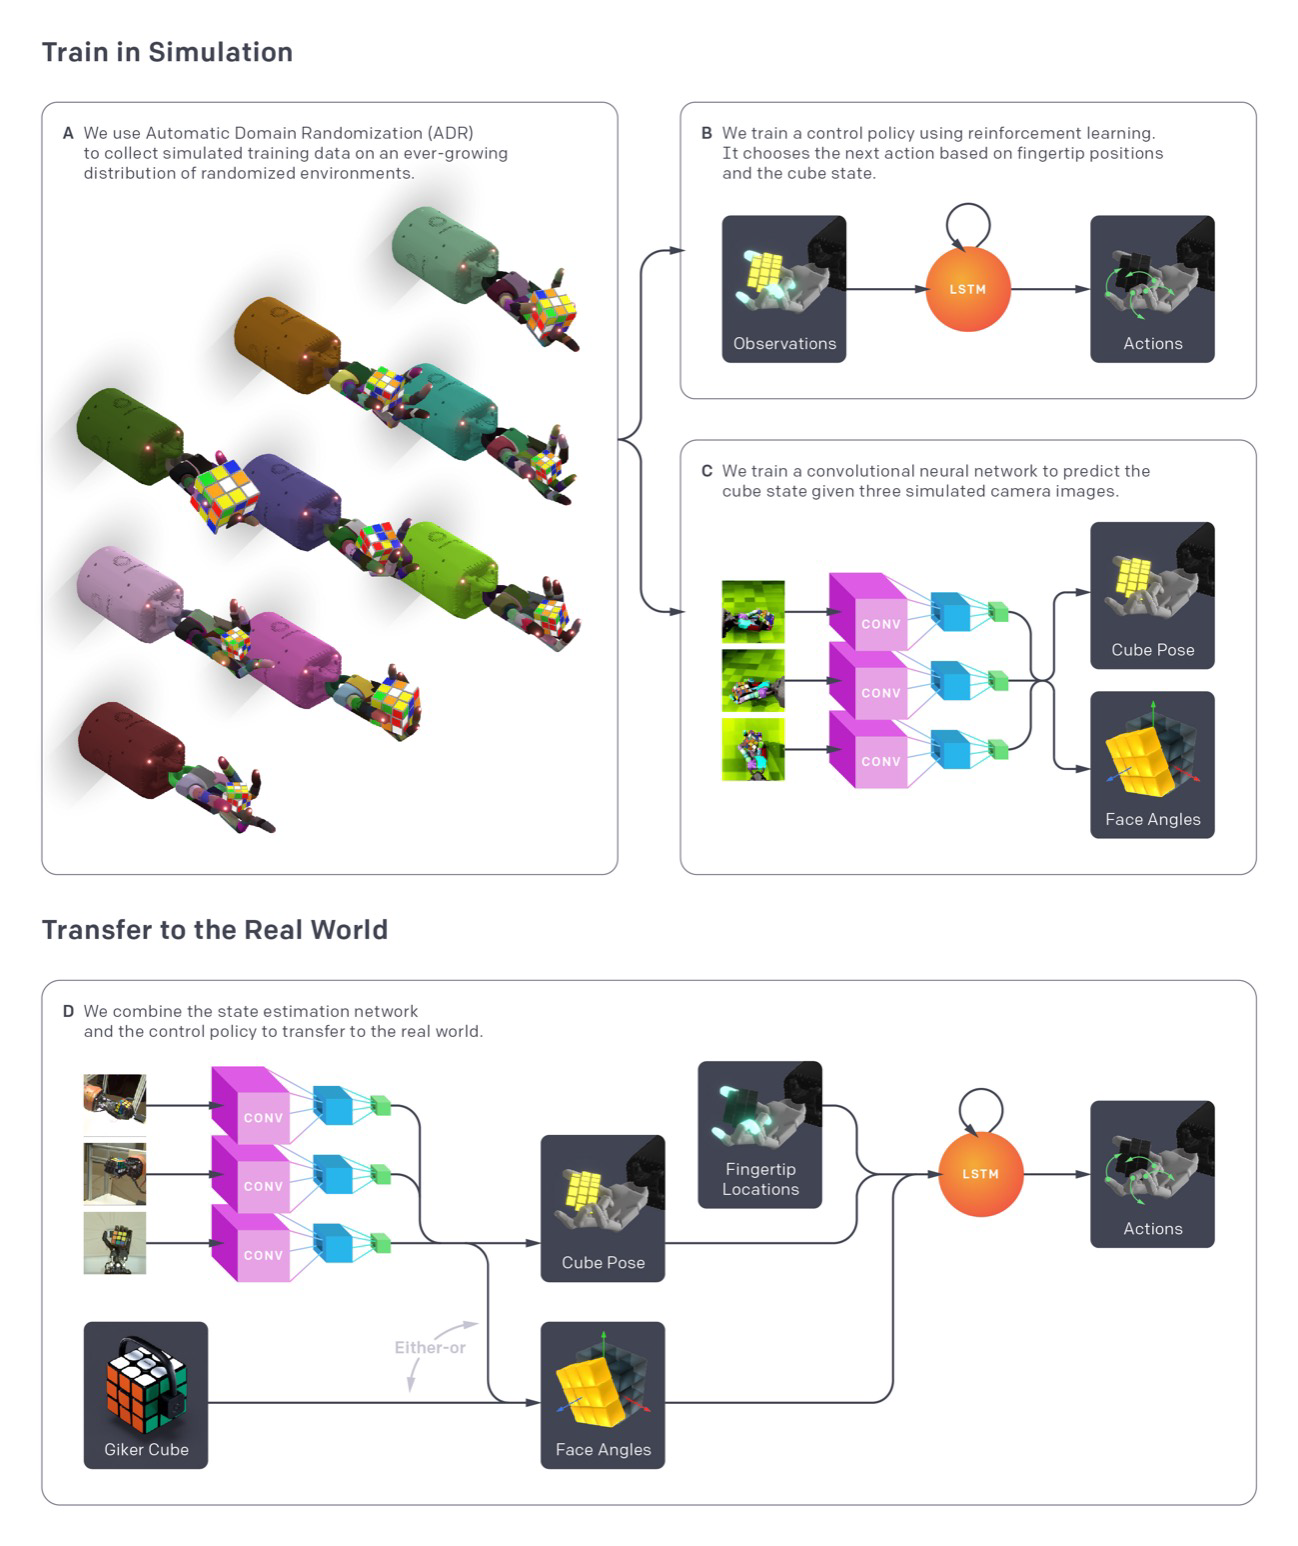
\includegraphics[width=0.95\linewidth]{figures/figAdrPipeline.png}
    \caption{Training pipeline with Automatic Domain Randomization (ADR) for \simtoreal transfer. (A) Simulation generates randomized cube-and-hand images; (B) a policy (LSTM) maps simulated observations (hand and cube states) to actions; (C) a CNN state estimator is trained to predict cube pose from images; (D) during real-world deployment, camera images pass through the CNN, then policy acts on estimated state. (\emph{Adapted from} Akkaya et al.~\cite{Akkaya2019}.)}
    \label{fig:adr_pipeline}
\end{figure}

\paragraph{Evaluation.} Domain randomization for visual perception has shown robust performance in tasks such as drone navigation (CAD2RL~\cite{Sadeghi2017}) and robotic manipulation (Dactyl~\cite{Akkaya2019}). In CAD2RL, this technique enabled quadrotors to more than double their collision-free flight-distance compared to a heuristic baseline (27.3 m vs. 12.5 m), while in Dactyl, vision-based manipulation improved from a median of 0 to over 11 successful cube rotations per episode \cite{Akkaya2019,Sadeghi2017}. Its main advantage is that it requires no real-world data and can be scaled easily. However, its effectiveness is sensitive to the diversity and realism of the randomized features. Over-randomization or unrealistic textures can degrade learning efficiency. Domain adaptation methods offer finer alignment but typically require real data and are challenging to scale to end-to-end RL pipelines~\cite{Tzeng2017}.

\section{Action-Level Transfer}

\section{Cross-Domain Case Studies}
To ground the above concepts, we now highlight several case studies where sim-to-real techniques have enabled successful transfer in different application domains. These examples span robotic manipulation, drone flight, and legged locomotion – demonstrating both the commonalities and unique challenges of each domain. Each case study will mention the task, the approach used to bridge the gap, and key results achieved on real systems.

\subsection{Robotic Object Manipulation}
One of the early triumphs of sim-to-real in RL was in robotic object manipulation – specifically, having robot arms or hands handle objects using policies learned in simulation. A representative example is object grasping and localization. In the 2017 study by Tobin et al. (discussed earlier in Domain Randomization), the task was for a robotic arm to pick up objects (toys of various shapes) on a table using input from an RGB camera. The challenge was primarily vision-based: the robot needed to perceive the objects’ positions and plan grasps. The researchers trained a convolutional neural network to detect object locations by training entirely on synthetic images of a cluttered tabletop with random textures, lighting, and distractor objects (domain randomization). Even though the simulated images looked nothing like the real world individually, the neural network learned to focus on geometric cues and was robust to color/texture. When this network was used on the real robot’s camera input, it localized objects with ~1.5 cm accuracy and enabled reliable grasping in the real world – all without any real-image training. This was a landmark result showing that simulation-only training could produce a useful real-world perception system for manipulation.

Building on that, OpenAI’s Dactyl (2018) tackled an even harder manipulation problem: dexterous in-hand manipulation. In that setup, a five-fingered robot hand had to reorient a block (and later a Rubik’s Cube) in its fingers. They trained the policy in a MuJoCo simulator with extensive randomizations of both visuals and physics (frictions, object mass, joint gains, etc.). One especially important aspect was using an LSTM (recurrent network) in the policy to allow it to adapt online to the physics – essentially the policy would “feel” how heavy or slippery the object was and adjust its strategy. This can be seen as a form of implicit system identification happening inside the policy’s hidden state (a clever trick). After training on on the order of $10^8$ timesteps (with massive parallelization), the policy was deployed to the real Shadow Hand. The result: the hand could successfully spin and reposition the block in precise ways, achieving the goal orientations consistently. Later, they even demonstrated the hand solving a Rubik’s Cube – an extremely complex manipulation – using the same policy architecture (with some additional state estimation help). The success of Dactyl was a strong validation of the domain randomization approach for high-dimensional control. Figure 3 shows the real robotic hand from the Dactyl system manipulating a block, an outcome of this sim-to-real training.

Another manipulation example is assembly tasks, such as inserting pegs or screwing in bolts. These tasks require fine precision and often have contact-rich dynamics (which simulators struggle with). In 2019, researchers at NVIDIA (Mahler et al., 2019) showed that by using a high-fidelity simulator (Isaac Gym) and randomizing friction and part tolerances, a policy could learn to insert a peg into a hole in sim and then perform it on a real robot arm with high success. They also leveraged domain adaptation by using depth camera inputs (which are easier to match between sim and real than RGB images). Depth images from simulation are quite comparable to real depth sensor data, so the gap was smaller; in some sense, choosing the right sensing modality (depth over RGB) is also a strategy to ease sim-to-real.

To summarize the manipulation domain: Visual randomization has been critical for perception-driven tasks, and dynamics randomization plus recurrent policies or system ID has been important for contact-rich tasks. These strategies enabled policies trained in simulation to achieve real-world feats like multi-object grasping and dexterous hand manipulation, which are significant milestones in robotics. Even so, challenges remain, such as more complex object interactions, generalizing to novel objects not seen in simulation, and long-horizon manipulation sequences. Current research is exploring combining imitation learning from a few real demos with simulation training to handle those cases (so that the policy gets a hint of real-world behavior to anchor it).

\subsection{Drone Navigation (UAV Flight)}
Unmanned aerial vehicles (UAVs or drones) present a compelling application for sim-to-real RL because crashing a real drone during learning is very costly, yet drones operate in highly dynamic environments where a robust policy is needed. The case study of CAD2RL by Sadeghi and Levine (2016) is instructive. They wanted a drone to perform collision avoidance in indoor hallways using only a single camera image as input (no fancy laser sensors). They trained a deep RL policy in a 3D simulator that generated random hallway textures and layouts – essentially the drone learned to react to visual input to avoid walls. Crucially, the network was never shown a real image during training, only the randomized simulated images. When they flew the policy on a real drone (a small quadrotor with an onboard camera), it was able to traverse real hallways and avoid obstacles for hundreds of meters of flight, all without collisions. This zero-shot transfer was achieved primarily by domain randomization of the visual domain (wall colors, pictures on the wall, floor patterns, lighting, etc.), so the drone didn’t overfit to any particular appearance. The dynamics in that case were less of an issue because the policy was high-level (it output velocity commands); a low-level stabilizing controller was running on the drone to handle basic flight, which is common in such setups.

Another example in drone navigation is in outdoor flight or in simulated city environments. Researchers have used simulators like Microsoft AirSim or Gazebo to train drone policies for tasks like following roads or avoiding moving obstacles. Domain adaptation has been applied here by taking simulated images (which might, for instance, not perfectly capture the complexity of natural outdoor scenes) and using neural networks to enhance realism. For instance, one could train a network to translate simulated aerial images to look like real aerial images using satellite photo datasets. By doing so, an RL agent trained on the translated images would be more familiar with real visuals when deployed.

One of the challenges unique to drones is the dynamics: unlike many ground robots, drones have very fast dynamics and are quite sensitive to aerodynamic effects (propeller wash, wind) which are hard to simulate exactly. Some recent works (2019–2021) have started to incorporate dynamics randomization for drones – e.g., randomizing the mass of the drone, motor thrust curves, latency in control signals, and wind disturbances during training. Combined with PID controllers or adaptive control on the drone, this has improved success in transferring agile flight maneuvers from simulation to real quadrotors. For example, if a simulated drone can learn to do a flip or a fast turn in the presence of random gusts of wind and motor power variations, the resulting policy is more likely to work on a physical drone where those factors occur naturally.

In summary, for drone navigation, vision-based tasks have benefited hugely from visual domain randomization (as in CAD2RL), while highly dynamic tasks require careful system identification (tuning simulators for drone dynamics) and possibly domain randomization of dynamics. Safety is a big concern – unlike a robot arm that might just miss a grasp, a bad drone policy can crash the vehicle. So often a conservative approach is used: the RL policy might be given to the real drone only when a safety controller can take over if it diverges, or training might happen progressively (low-speed flight policies then increasing speed). This relates to future directions in safe RL, but it’s worth noting as a practical aspect of sim-to-real for UAVs.

\subsection{Legged Robot Locomotion}
Legged robots, such as bipeds or quadrupeds, have high degrees of freedom and complex contact dynamics with the ground. They are an excellent testbed for sim-to-real because falls or instability in the real world are potentially damaging, yet simulation of legged locomotion can be made quite realistic with modern physics engines. One prominent case study is deep RL for quadruped locomotion by Tan et al. (2018). In that work, the task was to make a quadruped robot (with four legs, similar to MIT’s Mini Cheetah or Unitree’s Laikago) learn to trot and gallop – gaits that require dynamic balance. They used a combination of system identification and domain randomization: first, they improved their simulator’s fidelity by identifying the robot’s motor model and sensor latency (the time delay between sending a command and the motor responding, and between an event and the sensor reading). This alone significantly narrowed the gap because a lot of control policies are sensitive to latency. Next, they applied dynamics randomization during training: they varied parameters like friction coefficients of the feet and ground, small variations in motor torque output, and they even added random pushes to the robot in simulation to teach it to recover balance. They also constrained the observation space to be something the real robot could reliably sense (e.g., using on-board inertial measurements rather than assuming access to global orientation). With these measures, they trained a policy (using PPO) in simulation that could produce fast trotting and galloping gaits.

The result was that when this policy was deployed on the real quadruped robot, it could execute the learned gaits and remain stable, without any additional training on the robot. The robot achieved a trot at around 0.5 m/s and a galloping gait faster than that, which was quite an achievement at the time for learned controllers. The sim-to-real transfer here crucially depended on both identification (to get the simulator close, e.g. matching the real motor dynamics) and randomization (to account for remaining discrepancies, like a slightly different friction on the lab floor versus the sim). If they had trained only on a nominal simulator, small unmodeled effects could have led to the robot tripping or oscillating. Because the policy had experience with those perturbations (random pushes, etc.), it was robust.

Following this, many other works came out applying similar ideas to different robots. For instance, Hwangbo et al. (2019) trained a bipedal robot to jump and run using an accurate simulator and randomizing ground compliance (how springy the ground is), which let the robot handle both hard flooring and softer mats in reality. The theme is consistent: identify what matters, randomize the rest. Another interesting case was by Muratore et al. (2021) on a ball-in-cup task with a robot arm (a task where the robot must swing a cup to catch a ball on a string). They used dynamics randomization with adaptive feedback, meaning the policy had parameters that could adjust based on observed behavior differences, effectively learning a form of online system ID (this blurs into meta-learning territory). The policy learned to compensate for slightly different string lengths and ball weights between sim and real, successfully performing the trick on real hardware.

For legged locomotion, another challenge is often the computational cost: simulation of many-legged robots with contact can be slow. This is where tools like Isaac Gym’s massive parallelism have helped. Researchers have shown that you can train a policy for a simple biped to walk in just a few minutes using thousands of parallel simulations – a case of brute force enabled by GPUs. Once trained, transfer still needs the above techniques, but the training turnaround is faster.

To sum up the locomotion case: It highlights the importance of physics-side alignment. Visual realism is usually not an issue (these policies often don’t rely on external cameras, but on internal sensors like joint encoders, IMUs, etc.). Instead, it’s all about dynamics: masses, friction, delays, and unexpected forces. By addressing those through system identification and domain randomization, researchers have achieved robust locomotion controllers via deep RL that operate on real legged robots – something that even a few years ago was very difficult. Still, open problems include handling environment changes (e.g., different terrains like slippery ice or tall grass – one can randomize terrain properties to an extent, but extreme changes may need on-the-fly adaptation) and multi-contact scenarios (like a humanoid climbing or using

\subsection{(continued) Legged Locomotion (cont.)}
...multi-contact scenarios. For example, getting a bipedal humanoid to not only walk but also climb or use its arms for support involves complex interactions that are hard to simulate perfectly. Current sim-to-real techniques have yet to fully conquer these extreme cases, and they remain active research problems.
\section{Challenges and Future Directions}
Despite significant progress, sim-to-real transfer in reinforcement learning still faces numerous challenges. We highlight some key limitations and promising directions for future research:

\begin{enumerate}
    \item Simulator Fidelity vs. Generalization: Achieving a highly accurate simulator via system identification can be time-consuming and still incomplete – some aspects of reality (like subtle wear or complex contacts) resist exact modeling. On the other hand, relying on broad randomization without understanding can make training inefficient. A theoretical understanding of why domain randomization works and how to choose optimal randomization distributions is still lacking. Bridging this gap requires new insights. Future work may involve differentiable simulators or learned simulators that can be directly tuned with gradient-based methods, providing a more automated way to improve fidelity.
    \item Sample Efficiency and Real Data Usage: Many sim-to-real successes (e.g. OpenAI’s results) required an enormous amount of simulated experience, which is computationally expensive. While simulation is cheaper than real life, training might still take days or weeks on clusters. An open challenge is improving sample efficiency so that policies can learn robustly with less data. Techniques like model-based RL, which learn a model of the environment and plan with it, or offline RL using logged data, could reduce the need for brute-force simulation. Additionally, using small amounts of real data in the training loop can dramatically help but needs careful integration. Future systems might do real-to-sim-to-real loops where occasional real trials are used to correct the simulator (via system ID) or fine-tune the policy, thus continually reducing the reality gap.
    \item Domain Adaptation Limits: Current domain adaptation methods mostly assume a shared feature space or visual similarity between sim and real. In cases where the simulation and reality have fundamentally different observables (for instance, if a simulation provides full state info that a real robot can’t sense directly), adaptation is non-trivial. Also, training GANs or adaptation models can be unstable. There is room for more robust adaptation techniques, possibly using architectures that incorporate physical constraints or semantic information (e.g., ensuring that “objects” in a scene remain consistent through the translation). Future research could explore one-shot adaptation, where the policy adapts on the fly from the first few real observations – a bridge towards meta-learning.
    \item Safety and Exploration in the Real World: One reason we use simulation is to avoid unsafe explorations on real robots. However, when deploying the learned policy, there is still a risk if the policy encounters states it wasn’t prepared for. Ensuring safety during deployment (and during any real-world fine-tuning) is paramount, especially in domains like autonomous driving or healthcare. This calls for safe reinforcement learning approaches to be combined with sim-to-real. For instance, one might enforce that the policy respects certain safety constraints by design (through reward shaping or a filter) so that even if the sim was imperfect, the real robot won’t take catastrophic actions. Another idea is to have an intermediary training phase in a controlled real setting (like a lab with safety harnesses for a robot) to verify and adjust the policy before full deployment.
    \item Combining Methods and Multimodal Transfer: As noted, the most successful strategies often mix techniques – e.g., calibrating some parameters (system ID), randomizing others, and possibly adapting visual inputs. Designing unified frameworks that can do all of the above automatically is an ongoing direction. Recent work on adaptive domain randomization tries to learn the randomization range itself (using algorithms that adjust the randomization to where the policy is weak, focusing training on those). Moreover, integrating sim-to-real with other forms of transfer learning like imitation learning or human demonstrations is promising. A human demonstration in the real world could be used to guide the simulation randomization (to ensure the simulator produces similar scenarios) or to initialize the policy via imitation, after which RL in sim fine-tunes it. This can dramatically cut down training time and yield more human-compatible behaviors.
    \item Meta-Learning and Online Adaptation: One exciting avenue is meta-learning, where the policy is trained to adapt quickly to new environments. In a sim-to-real context, one could meta-train a policy across many simulated variations so that it can infer the current environment’s quirks (friction, weight, etc.) from a small amount of experience and adjust its behavior. This is related to what the recurrent policies (like the LSTM in Dactyl) are doing – implicitly identifying the environment. Future work could make this more explicit and efficient, perhaps by having a small network (an adaptation module) that updates some policy parameters using a few real-world trials. Such approaches blur the line between training and deployment, as the robot continues learning (or at least calibrating) once it’s in the real world. This can make the transfer more robust to long-term changes (like battery aging or component wear).
    \item Wider Domains and Generalization: So far, sim-to-real RL has mostly been demonstrated on specific tasks. A long-term goal is generalist agents that can transfer knowledge from simulation to reality across a variety of tasks without retraining from scratch for each one. This might involve training large RL policies or models (perhaps inspired by large-scale unsupervised learning) in simulation on many tasks and then adapting them to real tasks with minimal real data. In addition, applying sim-to-real in domains beyond robotics – for instance, in economics or internet simulations to real markets, or in training assistants in virtual environments before deploying to real human interaction – are frontiers that present their own challenges of fidelity and human unpredictability.
\end{enumerate}

In summary, while sim-to-real in reinforcement learning has matured a lot, especially in robotics, there remains a rich landscape of research ahead. The combination of improving simulation fidelity, smarter training techniques, and clever adaptation algorithms will continue to push the boundary. The interplay of these methods – and ensuring theoretical understanding catches up with empirical success – will be key to making sim-to-real transfer more reliable and routine.
\section{Conclusion}
Simulation-to-real transfer enables reinforcement learning agents to leverage the best of both worlds: the abundance and safety of simulated training, and the authenticity of real-world deployment. In this paper, we reviewed how core RL principles and various transfer techniques come together to bridge the notorious reality gap. We discussed domain randomization, which broadens training conditions until reality is just another variation, domain adaptation, which tweaks observations or learned representations to eliminate visual or sensory discrepancies, and system identification, which tunes simulators to mirror reality as closely as possible. Through case studies in robotic manipulation, drone navigation, and legged locomotion, we saw these ideas in action – turning what were once simulation-bound successes into real-world achievements.

Sim-to-real in reinforcement learning has evolved from a niche endeavor to a flourishing area of research. Robots can now grasp, fly, and walk using brains baptized in virtual worlds. Yet, as we highlighted, challenges like achieving higher fidelity, ensuring safety, and reducing data requirements remain before sim-to-real becomes a plug-and-play tool. Encouragingly, many future directions are being actively explored: from algorithms that learn how to randomize or adapt (meta-learning, Bayesian randomization) to more encompassing frameworks that combine multiple techniques for maximum robustness. The continued development of better simulators (e.g., photo-realistic renderers, differentiable physics) and more powerful RL algorithms will further close the gap.

Ultimately, success in sim-to-real not only advances robotics and AI by saving time and resources, but it also opens the door to deploying learning agents in the physical world with confidence. As our simulators become more like sandboxes for training “digital athletes,” we can tackle increasingly complex real-world tasks with agents that have practiced extensively in simulation. The progress so far – from video-game trained policies now controlling real robots, to drones and quadrupeds mastering skills via virtual trial and error – offers a compelling preview of what’s to come. By continuing to refine these methods, we move closer to a future where learning in simulation and performing in reality is a seamless pipeline, empowering RL to drive innovations in robotics, autonomous vehicles, and beyond.
%----------------------------------------------------------------------------------------

\bibliographystyle{abbrv} % "abbrv" reference style
\bibliography{refs} % Entries are in the refs.bib file

%----------------------------------------------------------------------------------------

\end{document}
